\documentclass[12pt,a4paper]{article}

% ── Encoding & language ──────────────────────────────────────────────────────
\usepackage[utf8]{inputenc}
\usepackage[T1]{fontenc}
\usepackage[english]{babel}

% ── Layout ───────────────────────────────────────────────────────────────────
\usepackage[top=2.5cm, bottom=2.5cm, left=2.5cm, right=2.5cm]{geometry}
\usepackage{fancyhdr}
\setlength{\headheight}{14.5pt}
\pagestyle{fancy}
\fancyhf{}
\lhead{\small Università della Calabria}
\rhead{\small Data Warehouse and Visualization}
\cfoot{\thepage}
\renewcommand{\headrulewidth}{0.4pt}

% ── Graphics and tables ──────────────────────────────────────────────────────
\usepackage{graphicx}
\usepackage{booktabs}
\usepackage{array}
\usepackage{float}
\usepackage{caption}
\usepackage{subcaption}
\usepackage{xcolor}

% ── Hyperlinks ───────────────────────────────────────────────────────────────
\usepackage[colorlinks=true, linkcolor=blue, urlcolor=blue, citecolor=blue]{hyperref}

% ── Math ─────────────────────────────────────────────────────────────────────
\usepackage{amsmath}

% ── Code / LLM prompts ───────────────────────────────────────────────────────
\usepackage{listings}
\lstset{
  basicstyle=\small\ttfamily,
  breaklines=true,
  frame=single,
  xleftmargin=6pt,
  xrightmargin=6pt
}

% ── Highlight box for the LLM/AI-based interventions ─────────────────────────
\usepackage{tcolorbox}
\tcbuselibrary{breakable}
\newtcolorbox{aibox}[1]{
  breakable,
  colback=violet!5,
  colframe=violet!60!black,
  boxrule=0.8pt,
  arc=2pt,
  left=8pt, right=8pt, top=4pt, bottom=4pt,
  title={AI -- #1},
  fonttitle=\bfseries\color{white},
  coltitle=white,
  colbacktitle=violet!60!black
}

% ── Paragraph spacing ────────────────────────────────────────────────────────
\setlength{\parskip}{6pt}
\setlength{\parindent}{0pt}

% ── Image paths ──────────────────────────────────────────────────────────────
\graphicspath{{./dq_plot/}{./cleaned/}{./}{../../dq_plot/}{../../cleaned/}}

% ─────────────────────────────────────────────────────────────────────────────
\begin{document}
\thispagestyle{empty}

% ═══════════════════════════════════════════════════════════════════════════
%  TITLE PAGE
% ═══════════════════════════════════════════════════════════════════════════
\begin{titlepage}
  \centering
  \vspace*{4cm}
  {\LARGE\textbf{Data Warehouse and Visualization}\par}
  \vspace{0.8cm}
  {\large Analysis of Olist E-Commerce\par}
  \vspace{1.5cm}
  {\large Emanuele Colecchia\par}
  {\large Student ID: 276527\par}
  \vspace{0.5cm}
  {\ttfamily clcmnl02c06g317o@studenti.unical.it\par}
  \vspace{0.5cm}
  {\large Academic Year 2025/2026\par}
\end{titlepage}

% ═══════════════════════════════════════════════════════════════════════════
%  TABLE OF CONTENTS
% ═══════════════════════════════════════════════════════════════════════════
\tableofcontents
\clearpage

% ═══════════════════════════════════════════════════════════════════════════
%  1. DATA SOURCE AND REQUIREMENTS
% ═══════════════════════════════════════════════════════════════════════════
\section{Data source description and requirements analysis}

\subsection{Data source}

For this project I used the \textit{Brazilian E-Commerce Public Dataset} published by
Olist on Kaggle:

\begin{center}
  \ttfamily https://www.kaggle.com/datasets/olistbr/brazilian-ecommerce
\end{center}

Olist is a Brazilian marketplace that connects small sellers with the country's main
e-commerce platforms. The dataset holds around 100,000 real, anonymized orders placed
between 2016 and 2018, spread across nine CSV files (Table~\ref{tab:csv}). The code for
the whole project -- cleaning pipeline, ETL, and analysis scripts -- is on GitHub at
\url{https://github.com/emanuele-clc/olist-dwh}.

\begin{table}[H]
  \centering
  \caption{CSV files of the Olist data source}
  \label{tab:csv}
  \begin{tabular}{ll}
    \toprule
    \textbf{File} & \textbf{Content} \\
    \midrule
    \texttt{olist\_customers\_dataset.csv}         & Customer registry with geographic location \\
    \texttt{olist\_sellers\_dataset.csv}            & Seller registry with geographic location \\
    \texttt{olist\_orders\_dataset.csv}             & Orders with statuses and lifecycle dates \\
    \texttt{olist\_order\_items\_dataset.csv}       & Products purchased per order, with prices and shipping \\
    \texttt{olist\_order\_payments\_dataset.csv}    & Payment methods and amounts \\
    \texttt{olist\_order\_reviews\_dataset.csv}     & Customer reviews and ratings \\
    \texttt{olist\_products\_dataset.csv}           & Product catalog with dimensions and categories \\
    \texttt{olist\_geolocation\_dataset.csv}        & Geographic coordinates by postal prefix \\
    \texttt{product\_category\_name\_translation.csv} & Category translation from Portuguese to English \\
    \bottomrule
  \end{tabular}
\end{table}

\subsection{Preliminary requirements analysis}

The goal is a decision-support system for looking at how Olist's business is actually
performing. The main questions the warehouse needs to answer are:

\begin{enumerate}
  \item Which product categories bring in the most revenue, and how is that spread out
        geographically?
  \item How have sales moved over time -- are there clear seasonal peaks?
  \item How does customer satisfaction (review score) change depending on product
        category, Brazilian state, and seller?
  \item What share of orders arrives on time? What is the average delay, and how does
        it vary by area?
  \item Which payment methods do customers use most?
\end{enumerate}

To answer these we need the following \textbf{dimensions}: Time (daily, up to year),
Product (category and macro-category), Customer (city--state--region), Seller
(city--state), and Payment Method. The main \textbf{measures} are revenue, shipping
cost, number of items sold, review score, and delivery delay.

\textit{Implementation note: the \texttt{macro\_category} (Product) and \texttt{region}
(Customer) hierarchies appear in the conceptual DFM model but were not built into the
current star schema, because the source data does not include a
category-to-macro-category table or a state-to-region mapping. Every other dimension
and measure was fully implemented.}

% ═══════════════════════════════════════════════════════════════════════════
%  2. RECONCILED DATABASE SCHEMA
% ═══════════════════════════════════════════════════════════════════════════
\section{Reconciled Database Schema}

\subsection{Design choices}

Starting from the CSV files, I built a relational reconciled database that pulls the
source data together into one normalized, consistent schema. This reconciled database
represents the operational picture: integrated, consistent, correct, detailed -- ready
to be loaded into the warehouse through the ETL process.

Compared to the raw structure, I made three main changes:

\begin{itemize}
  \item added the derived fields \texttt{delivery\_lead\_days} and
        \texttt{delivery\_delay\_days} to the \texttt{Orders} table;
  \item added \texttt{product\_category\_name\_english} to \texttt{Products} by
        joining with the translation table;
  \item aggregated \texttt{Geolocation} down to one record per ZIP prefix, using the
        coordinate centroid and the most frequent city/state.
\end{itemize}

\subsection{Entity-Relationship Schema}

Figure~\ref{fig:er} shows the E/R schema of the reconciled database. It has eight entities: \texttt{Orders}, \texttt{Order\_Items}, \texttt{Customers}, \texttt{Sellers}, \texttt{Products}, \texttt{Payments}, \texttt{Reviews}, and \texttt{Geolocation}.

\texttt{Order\_Items} sits at the center, since it is where the main relationships meet: each row belongs to one \texttt{Orders} record (\textit{CONTAINS}, 1:n), points to one \texttt{Products} record (\textit{INCLUDES}, 1:n), and one \texttt{Sellers} record (\textit{SELLS}, 1:n). \texttt{Orders} in turn links to \texttt{Customers} through \textit{PLACES} (1:n), to \texttt{Payments} through \textit{PAID VIA} (1:n), and to \texttt{Reviews} through \textit{RATED IN} (1:n). Finally, \texttt{Geolocation} links to both \texttt{Customers} and \texttt{Sellers} through \textit{LOCATES} (1:n on \texttt{zip\_code\_prefix}) -- this is a partial FK, since 278 customer records (157 distinct ZIP codes) and 7 sellers have a ZIP code with no match in the geolocation table.

\begin{figure}[H]
  \centering
  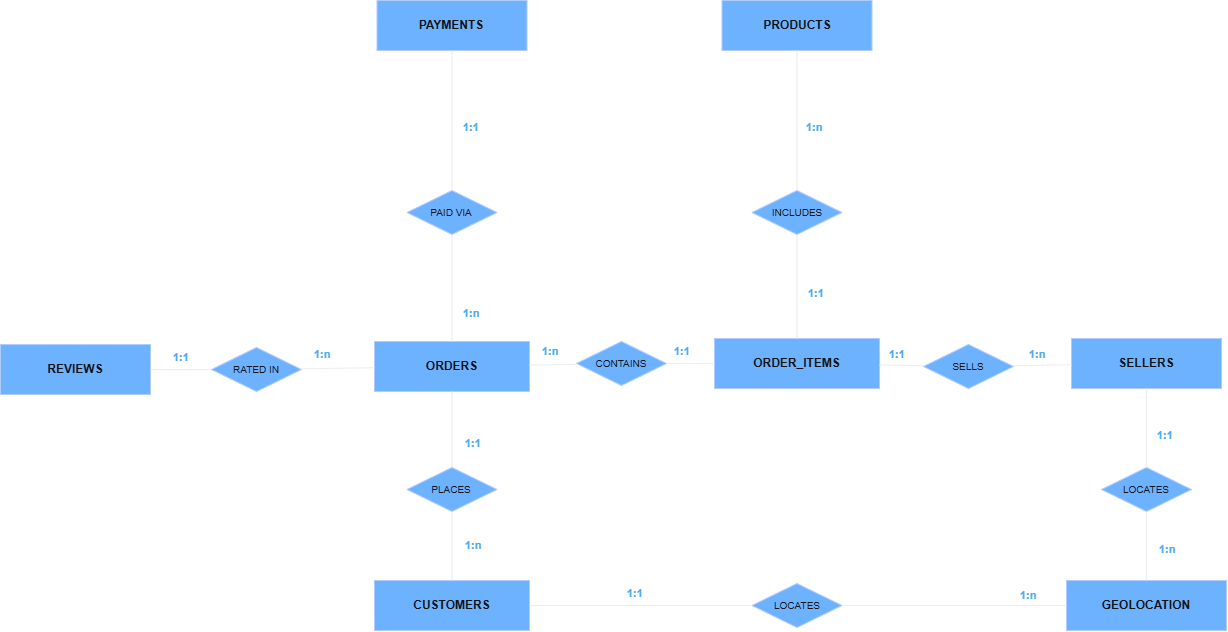
\includegraphics[width=\textwidth]{er_schema_pieno.png}
  \caption{E/R Schema of the Reconciled Database}
  \label{fig:er}
\end{figure}

\subsection{Relational Schema}

Below is the relational schema (primary keys underlined; asterisk = foreign key):

\begin{itemize}
  \item \textbf{Customers}(\underline{customer\_id}, customer\_unique\_id,
        zip\_code\_prefix*, city, state)\\
        \textit{\texttt{customer\_unique\_id} is the real, unique customer: the same
        person can show up under several different \texttt{customer\_id} values across
        orders. \texttt{zip\_code\_prefix} is a partial/optional FK to
        \texttt{Geolocation} (278 customer records, corresponding to 157 distinct ZIP
        codes, have no match in that table, so the join is a LEFT JOIN).}

  \item \textbf{Sellers}(\underline{seller\_id}, zip\_code\_prefix*, city, state)\\
        \textit{As with Customers, \texttt{zip\_code\_prefix} is a partial/optional FK
        to \texttt{Geolocation} (7 seller ZIP codes are missing, so again a LEFT
        JOIN).}

  \item \textbf{Products}(\underline{product\_id}, category\_name,
        category\_name\_english, name\_length, description\_length, photos\_qty,
        weight\_g, length\_cm, height\_cm, width\_cm)\\
        \textit{\texttt{category\_name\_english} comes from joining with the
        translation table.}

  \item \textbf{Orders}(\underline{order\_id}, customer\_id*, status,
        purchase\_timestamp, approved\_at, delivered\_carrier\_date,
        delivered\_customer\_date, estimated\_delivery\_date,
        delivery\_lead\_days, delivery\_delay\_days)\\
        \textit{\texttt{delivery\_lead\_days} and \texttt{delivery\_delay\_days} are
        computed during cleaning. They are NULL for orders that have not been
        delivered yet; I track that with separate binary flags.}

  \item \textbf{Order\_Items}(\underline{order\_id*, order\_item\_id}, product\_id*,
        seller\_id*, shipping\_limit\_date, price, freight\_value)\\
        \textit{Composite primary key, since one order can contain several products.}

  \item \textbf{Payments}(\underline{order\_id*, payment\_sequential},
        payment\_type, installments, value)\\
        \textit{An order can be split across multiple payment methods, hence the
        composite key with \texttt{payment\_sequential}.}

  \item \textbf{Reviews}(\underline{review\_id}, order\_id*, score, comment\_title,
        comment\_message, creation\_date, answer\_timestamp)\\
        \textit{Score is an integer from 1 to 5; the text fields are optional.}

  \item \textbf{Geolocation}(\underline{zip\_code\_prefix}, lat, lng, city, state)\\
        \textit{One geographic centroid per postal prefix -- the result of the per-ZIP
        aggregation done during cleaning.}
\end{itemize}

% ═══════════════════════════════════════════════════════════════════════════
%  3. DATA QUALITY ASSESSMENT AND DATA CLEANING
% ═══════════════════════════════════════════════════════════════════════════
\section{Data Quality Assessment and Data Cleaning}

\subsection{Methodology}

All the cleaning happens in a Python notebook
(\texttt{olist\_dw\_cleaning\_pipeline.ipynb}), built as a modular, auditable
pipeline. Every transformation step writes an entry to a global audit log, recording
table, operation, rows before/after, number of changes, and a short note on why.

I followed the usual data quality stages: \textbf{profiling} the raw data,
\textbf{spotting issues} with a programmatic scorecard, \textbf{classifying} them, and
then \textbf{fixing} what could be fixed, followed by a check that the fix actually
worked.

\subsubsection*{Classification of data quality issues}

Data quality issues fall into these categories:

\begin{itemize}
\sloppy
  \item \textbf{Missing values}: values that should be there but are not. Worth
        distinguishing from \textit{semantic nulls}, which are legitimately absent
        (e.g.\ a delivery date for an order that has not been delivered).
  \item \textbf{Wrong values}: values that exist but fall outside what is expected
        (e.g.\ \texttt{customer\_zip\_code\_prefix} truncated to 4 digits because a
        leading zero got dropped, or coordinates outside Brazil's geographic range).
  \item \textbf{Noisy data}: values that are technically valid but look odd
        statistically -- a simple domain rule cannot catch them; identifying them
        requires looking at the distribution (variance, standard deviation,
        mean~$\pm 3\sigma$, etc.).
  \item \textbf{Broken attribute dependencies}: values that break a functional
        dependency inside the same record (e.g.\ \texttt{approved\_at} coming before
        \texttt{purchase\_timestamp}).
  \item \textbf{Duplicate records}: several rows describing the same real-world
        thing, whether or not the values match exactly.
  \item \textbf{Inconsistent representations}: the same concept written in different
        ways (e.g.\ ``são paulo'' vs.\ ``São Paulo'').
\end{itemize}

\subsubsection*{Data quality indices}

For every dataset I measured five quality indices:

\begin{itemize}
  \item \textbf{Validity}: percentage of values respecting the declared domain rules
        (type, range, whitelist), calculated per attribute.
  \item \textbf{Completeness}: percentage of non-null values among the mandatory
        attributes. Optional attributes are left out so they do not skew the number.
  \item \textbf{Uniqueness}: percentage of records that are not duplicates of the
        primary key.
  \item \textbf{Consistency}: percentage of records that respect the declared
        dependencies between attributes.
  \item \textbf{Precision}: percentage of values that are not statistical outliers.
        For numeric columns this means the share within mean~$\pm 3\sigma$; for
        tables with no relevant numeric columns I just assume 100\%.
\end{itemize}

These indices come out of a programmatic scorecard (class \texttt{DQAReport}), driven
by rules I wrote for each attribute: Python lambdas for Validity, a list of mandatory
columns for Completeness, the key for Uniqueness, a list of dependencies for
Consistency. The scorecard gives an objective, repeatable view of quality, but it is
not the whole picture: noisy data does not show up in the Validity numbers when the
rule is loose (e.g.\ just \texttt{price > 0}), so the statistical distributions still
need to be checked by hand.

\begin{aibox}{Data Quality Assessment (L1) -- \texttt{10\_script\_llm}}
To help interpret the scorecard, I used \texttt{llama3.2:3b} through Ollama (running
locally, offline) as a narrative-analysis tool. For each table, I fed the pandas
statistical profile (null counts per column, duplicates, min/max/mean/std) into the
model with this prompt: \textit{``Analyze the data quality of this Olist table:
\{profile\}. For each issue indicate: DQ type, impact on the Data Warehouse,
recommended intervention.''}
This turned out useful where the scorecard alone was not enough: for Geolocation, the
model pointed out that the out-of-range coordinates might come from a systematic sign
error on longitude, which pushed me toward just filtering them out rather than trying
to fix them. For Reviews, it suggested checking the primary key on the pair
(\texttt{review\_id}, \texttt{order\_id}) instead of \texttt{review\_id} alone --
that one tip later led me to recover 814 legitimate records.
\end{aibox}

Table~\ref{tab:raw} shows the size of the source tables before I touched anything.

\begin{table}[H]
  \centering
  \caption{Sizes of the source tables (raw data)}
  \label{tab:raw}
  \begin{tabular}{lrrr}
    \toprule
    \textbf{Table} & \textbf{Rows} & \textbf{Total missing} & \textbf{Exact duplicates} \\
    \midrule
    Customers    &   99,441 &       0 &       0 \\
    Sellers      &    3,095 &       0 &       0 \\
    Products     &   32,951 &   2,448 &       0 \\
    Orders       &   99,441 &   4,908 &       0 \\
    Order Items  &  112,650 &       0 &       0 \\
    Payments     &  103,886 &       0 &       0 \\
    Reviews      &   99,224 & 145,903 &       0 \\
    Geolocation  & 1,000,163 &      0 & 261,831 \\
    \bottomrule
  \end{tabular}
\end{table}

\subsection{Detected issues and interventions}

\subsubsection{Customers (99,441 records)}

\begin{figure}[H]
  \centering
  
\includegraphics[width=0.9\textwidth]{dq_plot_customers.png}
  \caption{Data quality assessment -- \texttt{olist\_customers\_dataset}}
  \label{fig:dq_customers}
\end{figure}

Completeness, Uniqueness, and Consistency all sit at 100\%. The scorecard flags a
\textbf{Validity} problem (75.87\%), which comes entirely from
\texttt{customer\_zip\_code\_prefix}: the rule expects a numeric 5-digit ZIP, but
23,995 of 99,441 records (24.1\%) only have 4 digits, because the original CSV stores
this field as a number and drops the leading zero on ZIP codes starting with
\texttt{0} (a \textit{wrong values} issue). \texttt{customer\_state}, on the other
hand, already matches the \texttt{BR\_STATES} whitelist with zero invalid records --
the state codes were already uppercase in the source.

A manual look also turns up a second problem the scorecard does not catch, since
\texttt{customer\_city} has no domain rule attached to it: city names show up in
\textbf{inconsistent formats} (e.g.\ ``são paulo'' vs.\ ``São Paulo''). This is an
instance-level \textbf{Consistency} issue, and I handled it separately from the
scorecard.

\textbf{Fix -- automatic:} \texttt{str.strip()} on all text fields to remove stray
whitespace; \texttt{str.title()} on \texttt{customer\_city} (Consistency);
\texttt{str.upper()} on \texttt{customer\_state} as a precaution, to guarantee it
stays consistent even though it changed nothing in practice (0 records affected,
since everything already matched \texttt{BR\_STATES}).

\textbf{Result}: 99,441 records, 0 missing, 0 duplicates; Completeness, Uniqueness,
and Consistency at 100\%. The Validity issue on \texttt{customer\_zip\_code\_prefix}
(4-digit ZIP) is not fixed by the pipeline -- I left it as a documented known
limitation, since it has no real effect on city/state-level analysis.

\subsubsection{Sellers (3,095 records)}

\begin{figure}[H]
  \centering
  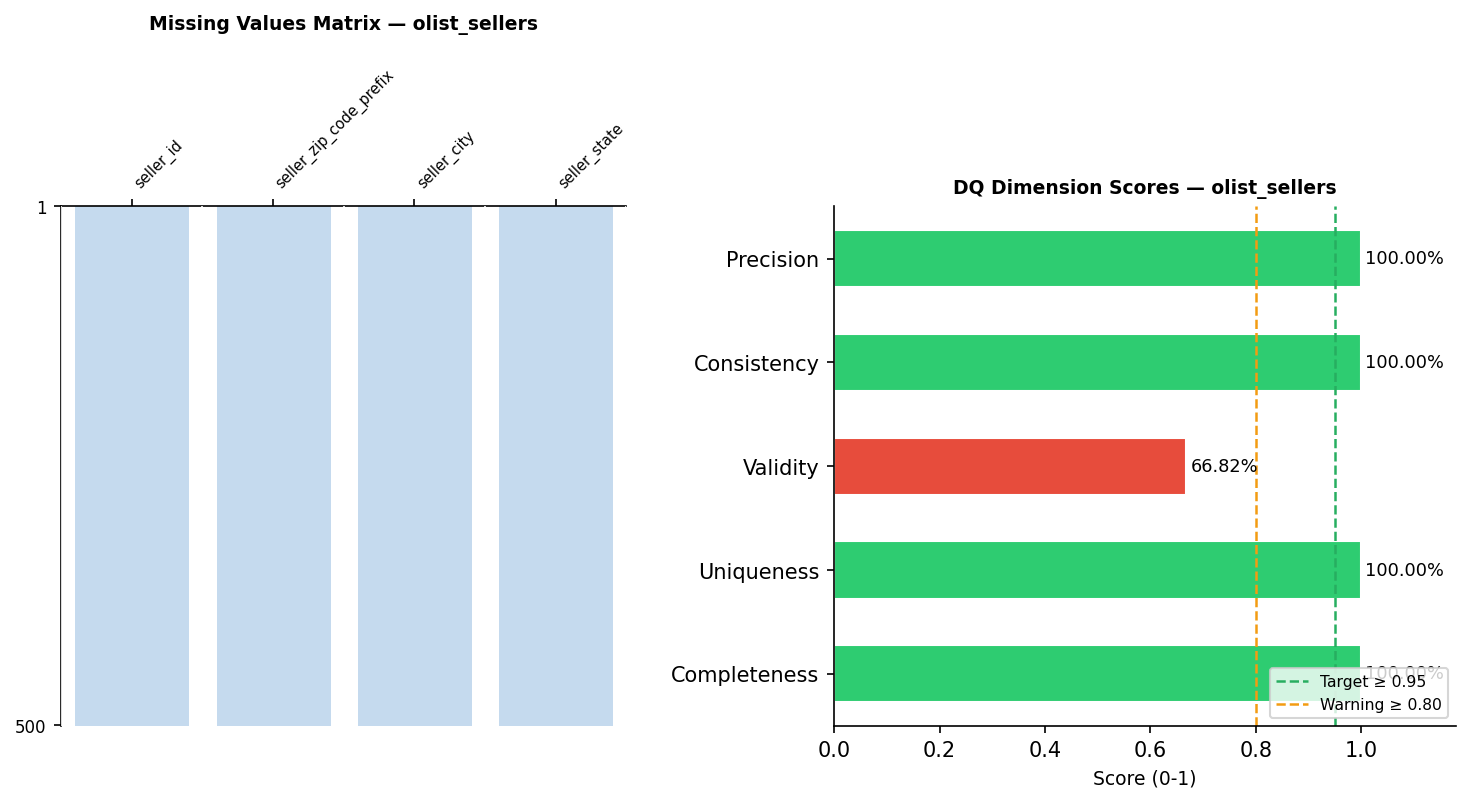
\includegraphics[width=0.9\textwidth]{dq_plot_sellers.png}
  \caption{Data quality assessment -- \texttt{olist\_sellers\_dataset}}
  \label{fig:dq_sellers}
\end{figure}

The situation closely mirrors Customers: the scorecard flags a \textbf{Validity}
issue (66.82\%) coming from \texttt{seller\_zip\_code\_prefix} -- 1,027 of 3,095
records (33.2\%) have a 4-digit ZIP for the same leading-zero reason.
\texttt{seller\_state} already matches \texttt{BR\_STATES} with zero invalid records
(already uppercase in the source). The manual check again finds inconsistent
formatting on \texttt{seller\_city}.

\textbf{Fix -- automatic:} \texttt{str.strip()} and \texttt{str.title()} on
\texttt{seller\_city} (Consistency); \texttt{str.upper()} on \texttt{seller\_state}
as a precaution (0 records actually changed).

\textbf{Result}: 3,095 records, 0 missing, 0 duplicates; Completeness, Uniqueness,
and Consistency at 100\%. As with Customers, the \texttt{seller\_zip\_code\_prefix}
issue stays as a documented, unfixed limitation.

\subsubsection{Geolocation (1,000,163 original records)}

\begin{figure}[H]
  \centering
  
\includegraphics[width=0.9\textwidth]{dq_plot_geolocation.png}
  \caption{Data quality assessment -- \texttt{olist\_geolocation\_dataset}}
  \label{fig:dq_geo}
\end{figure}

Two main problems show up here. First, a \textbf{Uniqueness} issue (58.84\%): the
same postal prefix appears with multiple different coordinates, giving 261,831
duplicate rows (26.2\%) -- this is \textit{record duplication}, since several records
describe the same real-world ZIP with different values. Second, a \textbf{Validity}
issue (75.43\%): some rows have \texttt{lat}/\texttt{lng} coordinates outside
Brazil's actual range ($lat \in [-33.75; 5.27]$, $lng \in [-73.99; -34.79]$) --
\textit{wrong values}.

\textbf{What I did:}
\begin{enumerate}
  \item Normalized the text in \texttt{city} and \texttt{state} (Consistency).
  \item Filtered out rows with out-of-range coordinates (Validity).
  \item Removed exact duplicates with \texttt{drop\_duplicates()} (Uniqueness).
  \item Aggregated by \texttt{zip\_code\_prefix}: averaged lat/lng into a centroid,
        took the most common city/state, and kept \texttt{n\_records} as a count of
        how many original points went into each prefix -- useful as a rough
        reliability signal for the centroid.
\end{enumerate}

\textbf{Result}: 19,015 records, 0 missing, 0 duplicates.

\subsubsection{Products (32,951 records)}

\begin{figure}[H]
  \centering
  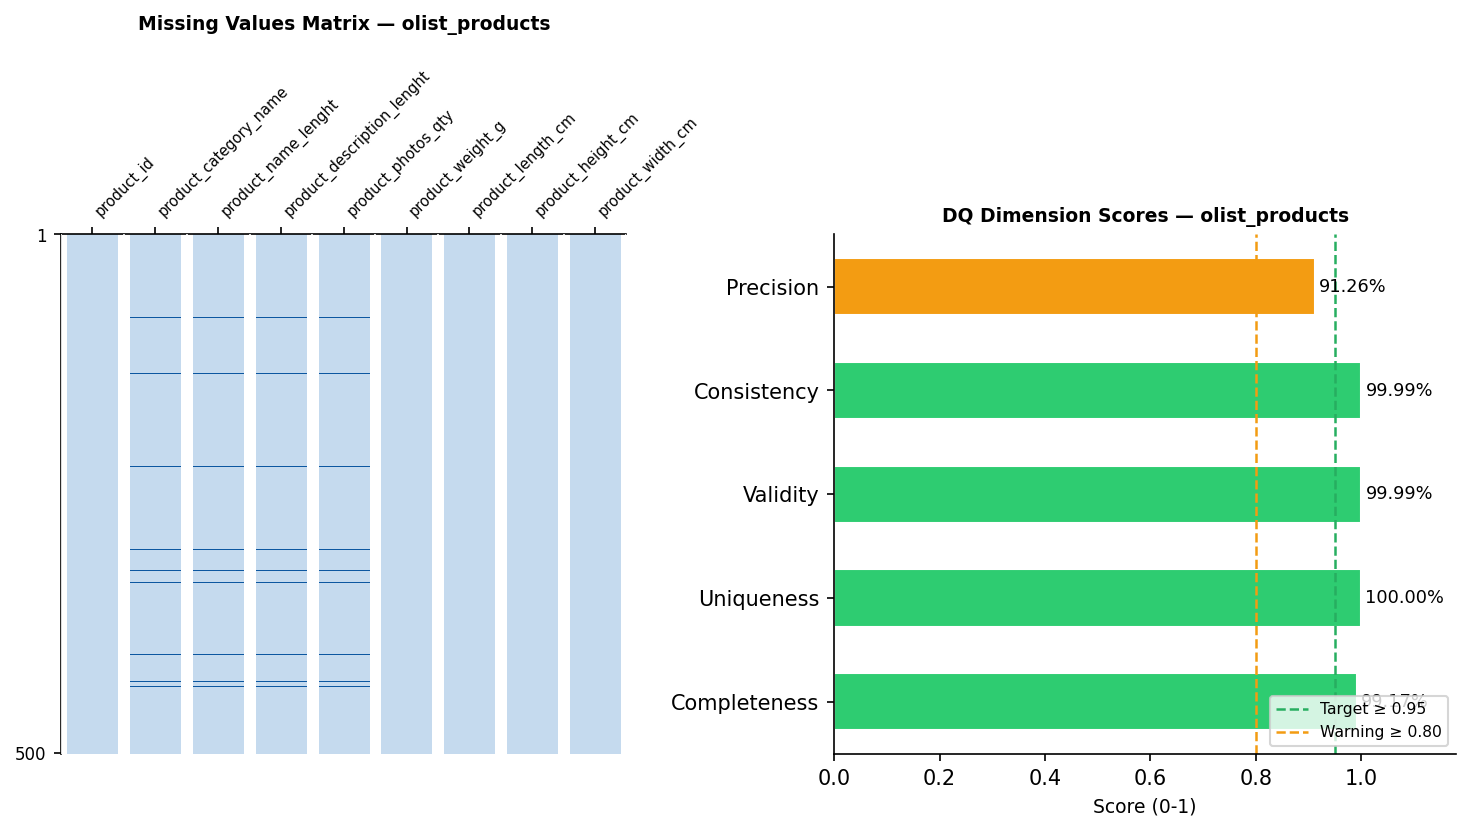
\includegraphics[width=0.9\textwidth]{dq_plot_products.png}
  \caption{Data quality assessment -- \texttt{olist\_products\_dataset}}
  \label{fig:dq_products}
\end{figure}

The scorecard puts \textbf{Completeness} at 99.17\%, due to 610 missing values in
\texttt{product\_category\_name} (1.85\%) plus some nulls in the physical columns
(weight, dimensions). Validity, Uniqueness, and Consistency are all close to 100\%.

Looking at the distribution of the physical measures also turns up a \textit{noisy
data} problem the scorecard misses, since the Validity rule only checks
\texttt{> 0}: values like a $40{,}000\,\text{g}$ weight or extreme dimensions pass
that check even though they are clearly off. These outliers still needed handling --
they count as \textit{noisy data / wrong values} in the course classification, even
if the scorecard cannot ``see'' them.

Note: the column names \texttt{product\_name\_lenght} and
\texttt{product\_description\_lenght} (missing the ``h'', a typo in the original
source) were kept as-is to stay compatible with the original schema.

\begin{aibox}{Missing Values \& Outlier Classification (L2) -- \texttt{10\_script\_llm}}
For classifying missing values as MCAR/MAR/MNAR, I used the LLM as decision support,
with this prompt: \textit{``For each column with nulls: classify as MCAR/MAR/MNAR
with justification, explain the impact on the DW, and indicate the recommended
imputation strategy.''}, fed with the missingness statistics computed in pandas.
Main takeaways: nulls in \texttt{product\_category\_name} were classified as
\textbf{MCAR} (uncatalogued products, no obvious pattern) $\to$ fill with the
constant \texttt{"unknown"}. Nulls in the physical measures as \textbf{MAR}
(products with an incomplete listing, correlated with having few photos) $\to$ fill
with the median, which holds up better than the mean when outliers are present.
Nulls in delivery dates as \textbf{semantic nulls} (orders not yet delivered) $\to$
no imputation, just a binary flag.
\end{aibox}

\textbf{What I did:}
\begin{enumerate}
  \item \textbf{Missing values} in \texttt{product\_category\_name} (Completeness):
        filled with the constant \texttt{"unknown"}, since there is no way to guess
        the real category without more information (the standard \textit{fill in
        with a global constant} technique from the course).

  \item \textbf{Missing values} in the physical numeric columns (Completeness):
        filled with the \textbf{median} computed over the valid records, since it is
        more robust to outliers than the mean. I added a binary \texttt{\_imputed}
        flag for each imputed column.

  \item \textbf{Noisy data} in the physical columns: flagged using the \textbf{IQR}
        method (lower bound $Q_1 - 1.5 \cdot IQR$, upper bound $Q_3 + 1.5 \cdot IQR$),
        with a binary \texttt{\_outlier} flag per column. Original values are kept in
        the reconciled database.

  \item Joined with the translation table to add
        \texttt{product\_category\_name\_english}.
\end{enumerate}

\textbf{Result}: 32,951 records, 0 missing, 0 duplicates. 22 columns total (9
original $+$ the English category $+$ 12 flags: 8 \texttt{\_imputed} and 4
\texttt{\_outlier}).

\subsubsection{Orders (99,441 records)}
\label{sec:orders-cleaning}

\begin{figure}[H]
  \centering
  
\includegraphics[width=0.9\textwidth]{dq_plot_orders.png}
  \caption{Data quality assessment -- \texttt{olist\_orders\_dataset}}
  \label{fig:dq_orders}
\end{figure}

The scorecard shows \textbf{Completeness} at 99.38\% and \textbf{Consistency} at
96.98\%, with Validity and Uniqueness both at 100\%. Precision is 100\% here too,
since there are no numeric columns with a relevant anomalous distribution -- the
``noisy'' cases in Orders are really about the date columns, and I already handle
those with semantic-null flags.

The null values in the date columns (160 in \texttt{order\_approved\_at}, 1,783 in
\texttt{order\_delivered\_carrier\_date}, 2,965 in
\texttt{order\_delivered\_customer\_date}) are \textbf{semantically correct}: they
simply mean the order was not approved or has not been delivered yet. They are not
real missing values and should not be filled in. The Consistency drop (96.98\%)
comes from 3,003 records that break at least one date dependency (e.g.\
\texttt{approved\_at} before \texttt{purchase\_timestamp}) -- a \textit{broken
attribute dependency} at the record level.

\textbf{What I did:}
\begin{enumerate}
  \item \texttt{str.lower()} on \texttt{order\_status} -- automatic fix (Consistency,
        representation level).
  \item \texttt{pd.to\_datetime()} on all date columns -- automatic fix (Validity:
        the timestamps were stored as plain strings).
  \item Added binary flags \texttt{\_approved\_missing},
        \texttt{\_delivered\_carrier\_missing},
        \texttt{\_delivered\_customer\_missing} to mark semantic nulls without
        filling them in.
  \item Kept the date-dependency violations in the reconciled database with their
        original timestamps (no imputation), but flagged them for later analysis.
  \item Feature engineering:
        \begin{itemize}
          \item \texttt{delivery\_delay\_days} $=$ actual delivery $-$ estimated
                delivery (negative $=$ early);
          \item \texttt{delivery\_lead\_days} $=$ actual delivery $-$ purchase date;
          \item \texttt{purchase\_year}, \texttt{purchase\_month} pulled from the
                purchase timestamp.
        \end{itemize}
\end{enumerate}

\textbf{Result}: 99,441 records, 0 duplicates. \texttt{NaN} values remain in the
derived columns for undelivered orders, as expected. 15 columns total.

\subsubsection{Order Items (112,650 records)}

\begin{figure}[H]
  \centering
  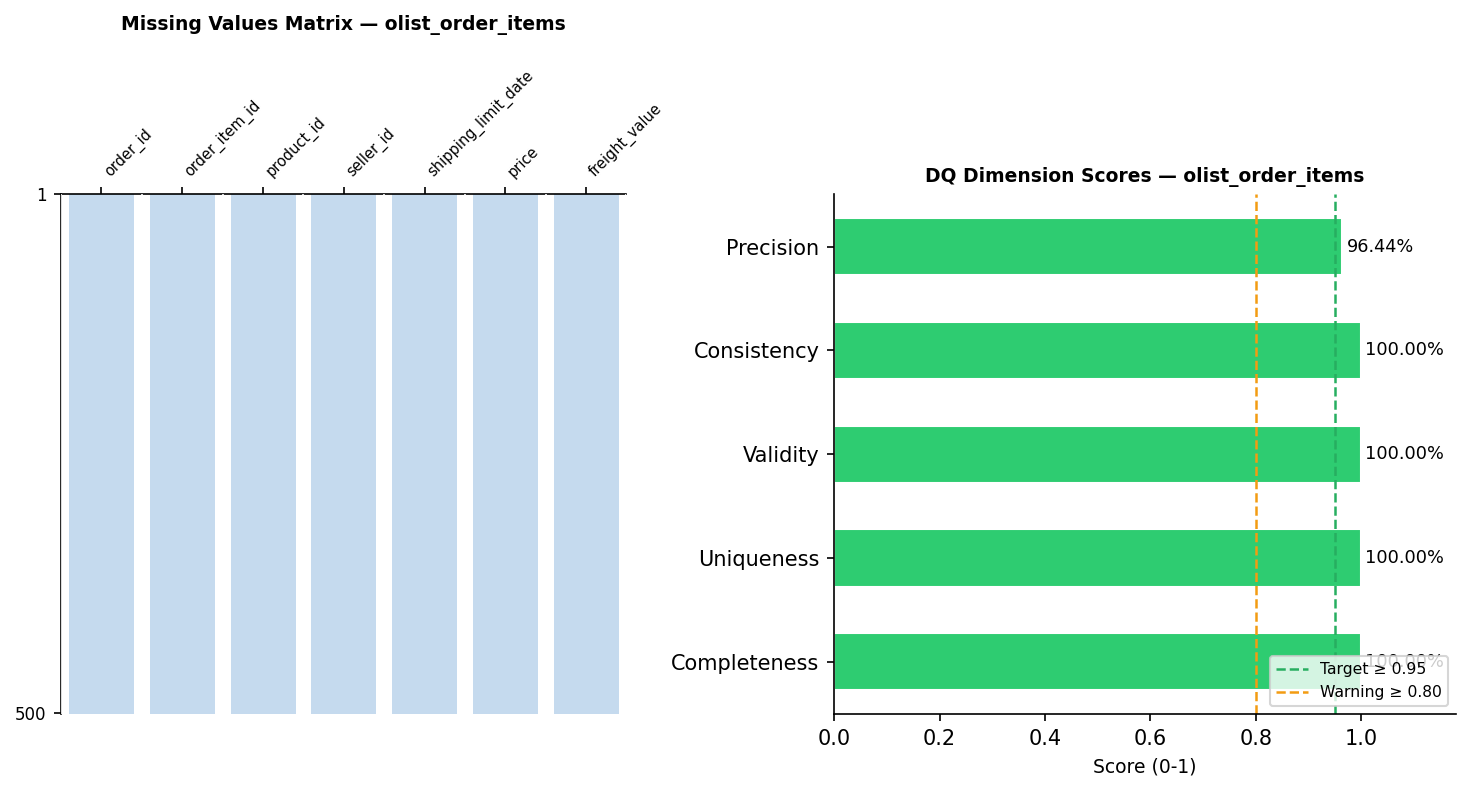
\includegraphics[width=0.9\textwidth]{dq_plot_order_items.png}
  \caption{Data quality assessment -- \texttt{olist\_order\_items\_dataset}}
  \label{fig:dq_items}
\end{figure}

Completeness, Uniqueness, Validity, and Consistency all sit at 100\%. Precision is
computed on \texttt{price}: the share of values within mean~$\pm 3\sigma$, which is
a rough indicator of noisy data.

Looking at how \texttt{price} is distributed turns up a \textit{noisy data} issue
the scorecard does not catch, since the Validity rule only checks
\texttt{price > 0}: every value is positive, but the distribution stretches up to
6,735 BRL with a long right tail. \texttt{freight\_value} shows the same pattern.
This is a good example of an issue that only shows up when looking at the
distribution, not with a simple pointwise rule -- \textit{noisy data / wrong values}.

\textbf{What I did:}
\begin{enumerate}
  \item \texttt{pd.to\_datetime()} on \texttt{shipping\_limit\_date} -- automatic
        fix (Validity).
  \item \textbf{Noisy data} on \texttt{price}: flagged with the \textbf{IQR} method
        ($Q_1 - 1.5 \cdot IQR$ / $Q_3 + 1.5 \cdot IQR$), binary
        \texttt{\_price\_outlier} flag added, original values kept.
  \item \textbf{Noisy data} on \texttt{freight\_value}: same approach,
        \texttt{\_freight\_value\_outlier} flag, original values kept.
\end{enumerate}

\begin{figure}[H]
  \centering
  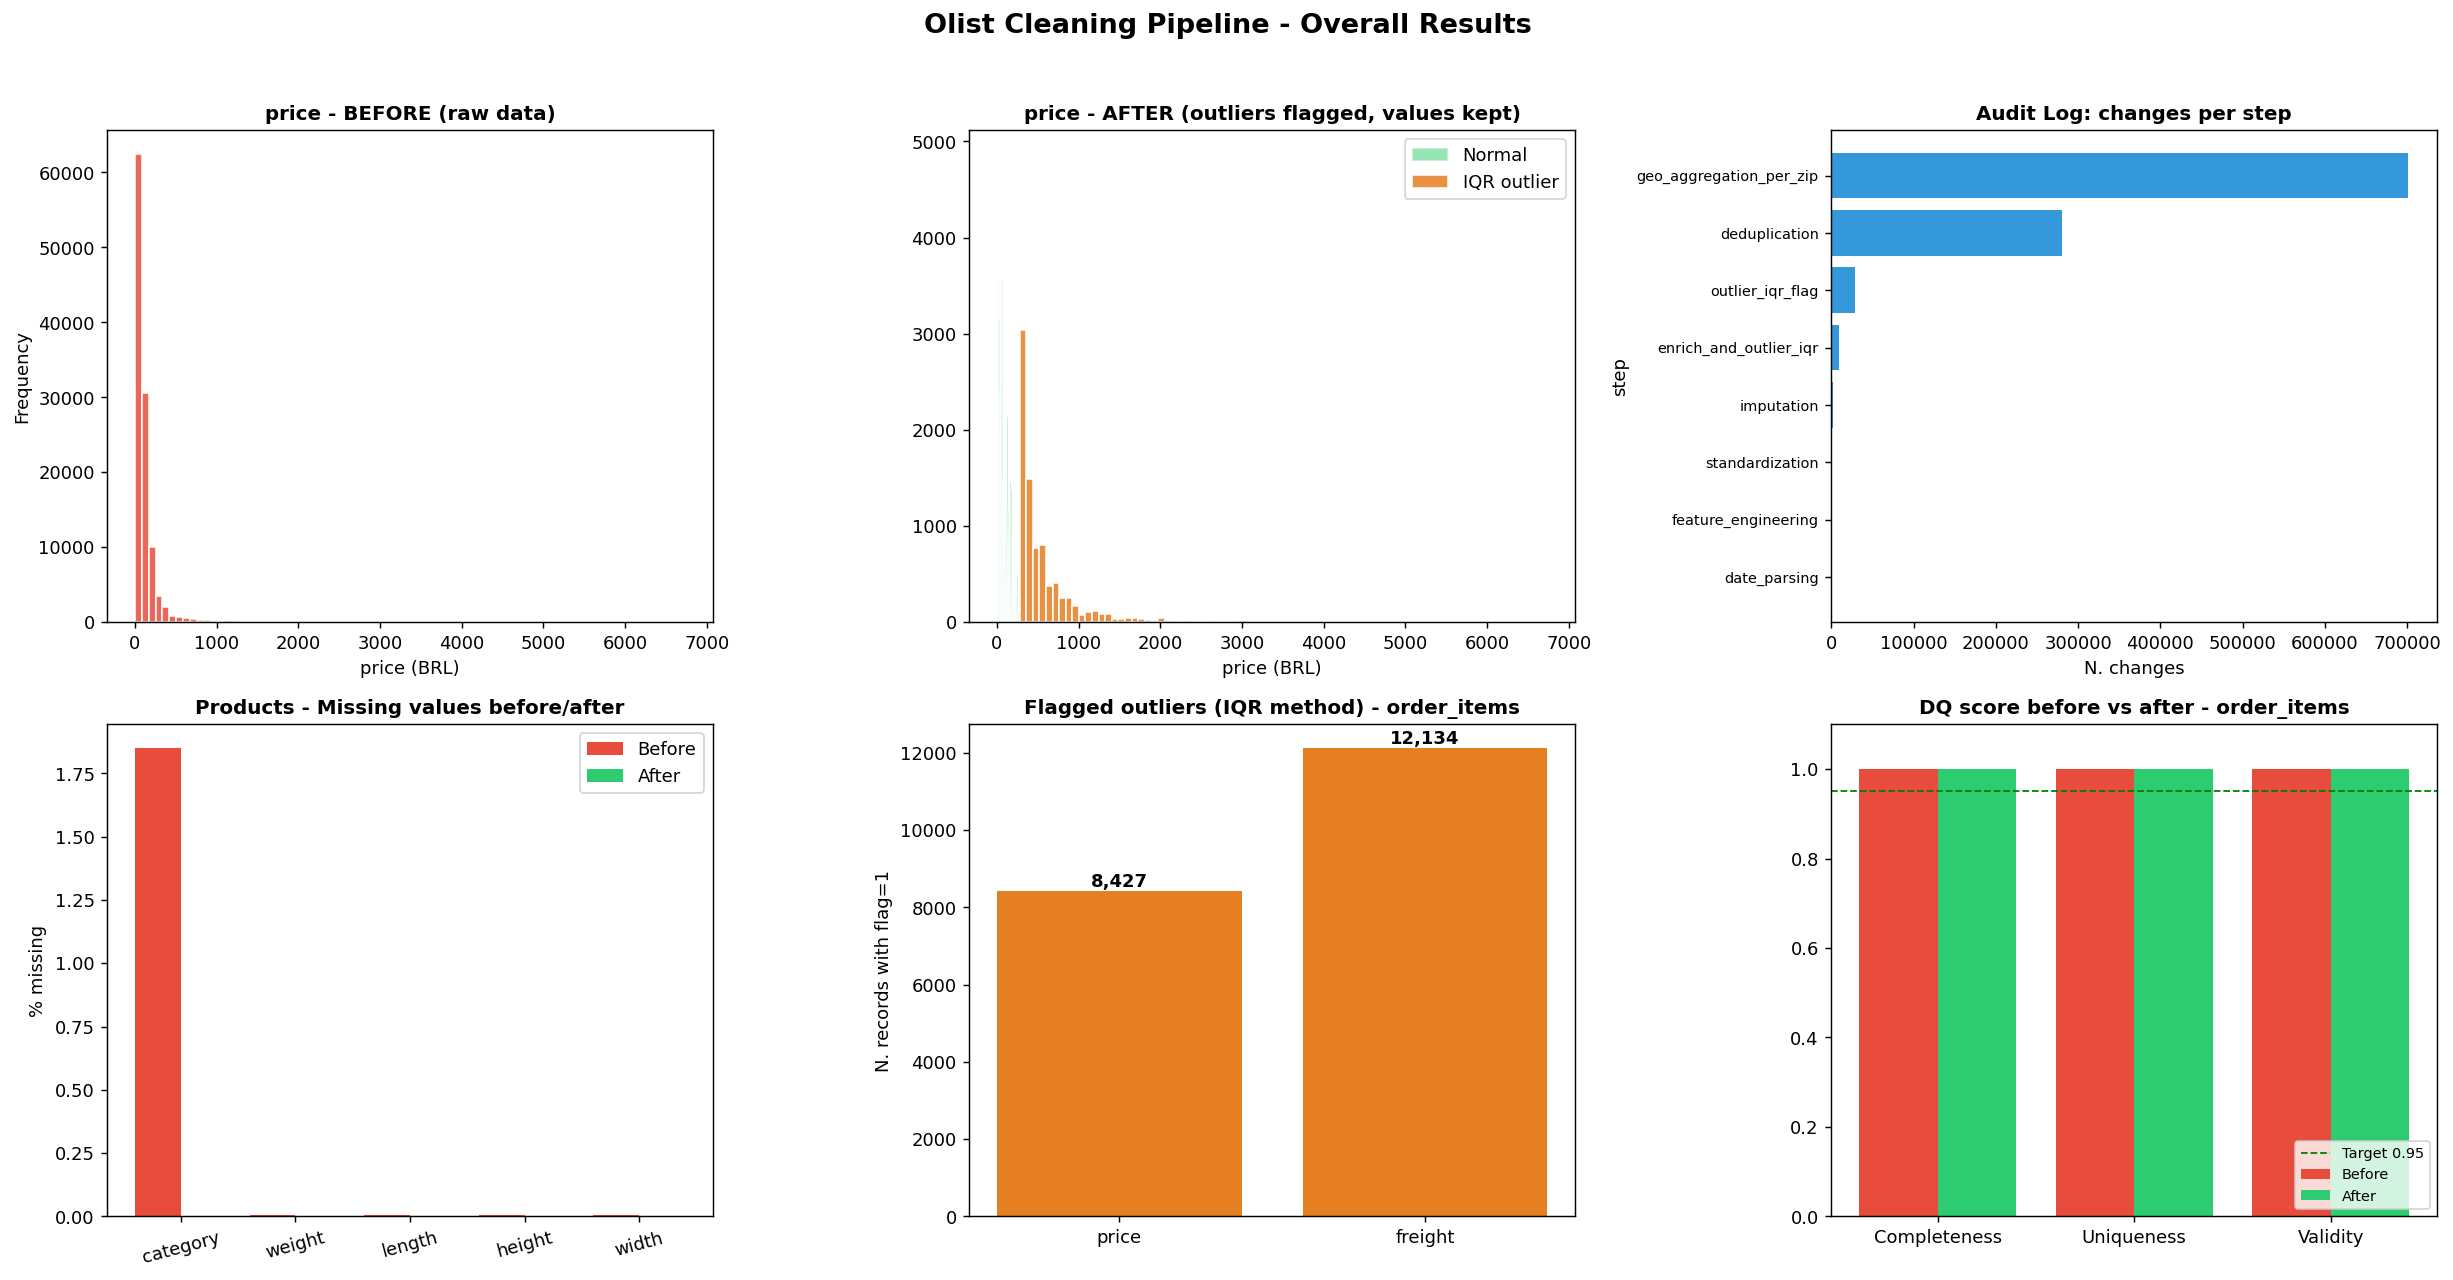
\includegraphics[width=\textwidth]{cleaning_pipeline_results.png}
  \caption{Overall results of the cleaning pipeline: price distribution before/after,
           audit log per step, missing values in Products, flagged outliers (IQR
           method) for \texttt{order\_items}, and DQ score before/after.}
  \label{fig:pipeline}
\end{figure}

\textbf{Result}: 112,650 records, 0 missing, 0 duplicates. 9 columns (7 original
$+$ 2 \texttt{\_outlier} flags).

\textit{Note: \texttt{total\_item\_value} $=$ \texttt{price} $+$
\texttt{freight\_value} is not stored in the reconciled database, since it is a
trivial derived value -- it gets computed directly in Tableau at visualization time.}

\subsubsection{Payments (103,886 records)}

\begin{figure}[H]
  \centering
  
\includegraphics[width=0.9\textwidth]{dq_plot_order_payments.png}
  \caption{Data quality assessment -- \texttt{olist\_order\_payments\_dataset}}
  \label{fig:dq_payments}
\end{figure}

All indices are at 100\% here. \texttt{payment\_type} has five values:
\texttt{credit\_card} (76,795, 73.9\%), \texttt{boleto} (19,784, 19.0\%),
\texttt{voucher} (5,775, 5.6\%), \texttt{debit\_card} (1,529, 1.5\%), and
\texttt{not\_defined} (3 records, 0.003\%). I kept those 3 \texttt{not\_defined}
records in the Validity whitelist -- the number is negligible and they could be
legitimate, just unclassified, transactions.

The same pattern shows up in \texttt{payment\_value}: the distribution has a long
right tail that the \texttt{>= 0} rule does not catch. I treated it the same way as
the order item prices.

\textbf{What I did:}
\begin{enumerate}
  \item \texttt{str.lower()} on \texttt{payment\_type} -- automatic fix
        (Consistency, representation level).
  \item \textbf{Noisy data} on \texttt{payment\_value}: flagged with the
        \textbf{IQR} method ($Q_1 - 1.5 \cdot IQR$ / $Q_3 + 1.5 \cdot IQR$) $+$
        \texttt{\_payment\_value\_outlier} flag, original values kept.
\end{enumerate}

\textbf{Result}: 103,886 records, 0 missing, 0 duplicates. 6 columns (5 original
$+$ 1 outlier flag).

\subsubsection{Reviews (99,224 records after cleaning)}

\begin{figure}[H]
  \centering
  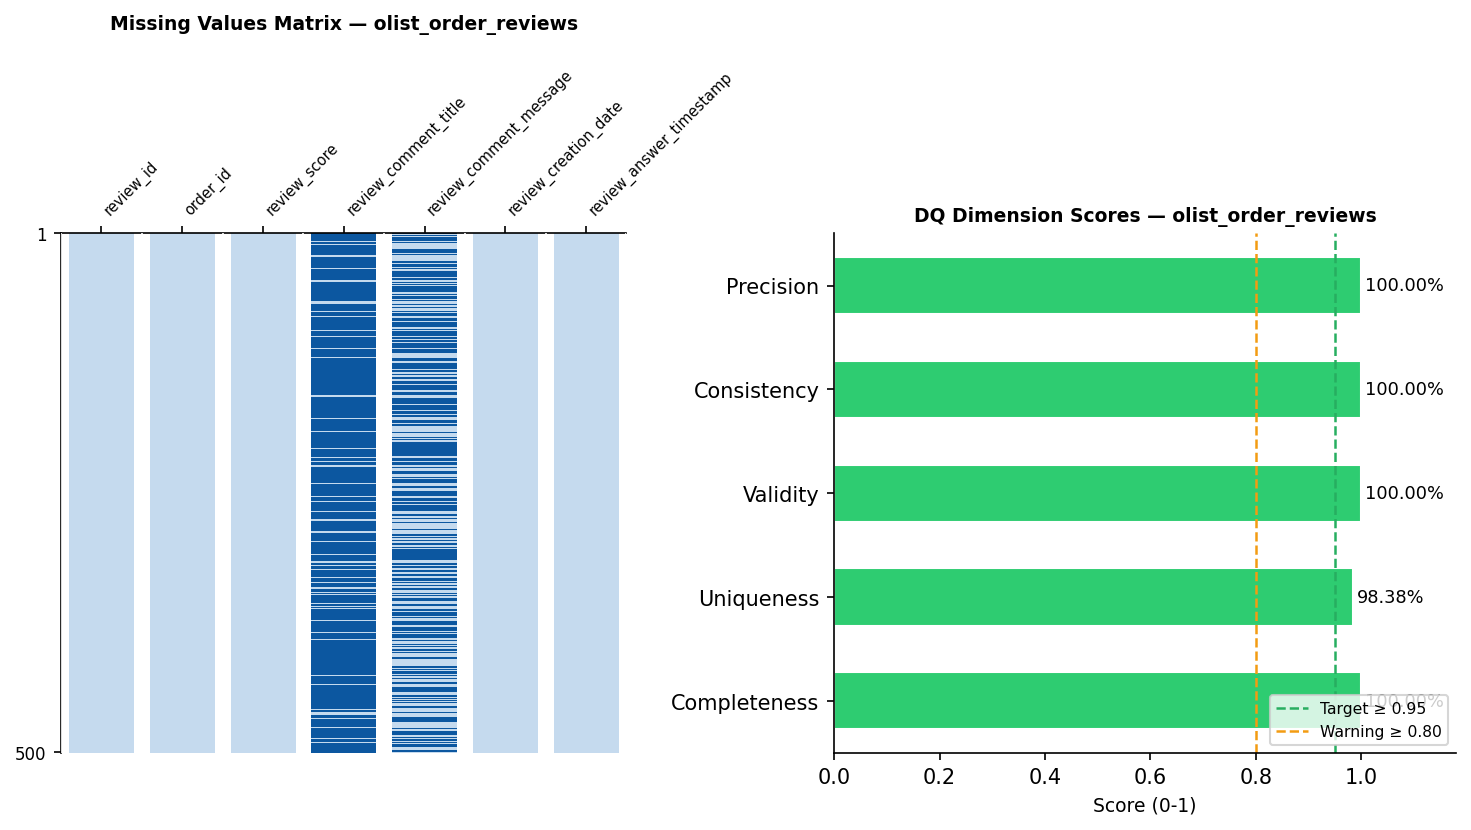
\includegraphics[width=0.9\textwidth]{dq_plot_order_reviews.png}
  \caption{Data quality assessment -- \texttt{olist\_order\_reviews\_dataset}}
  \label{fig:dq_reviews}
\end{figure}

With \texttt{review\_id} as the assumed primary key, the scorecard shows
\textbf{Uniqueness} at 98.38\% -- 1,603 records share a repeated \texttt{review\_id},
814 of them beyond the first occurrence. Validity and Completeness are both at 100\%.

A closer look shows these are not actually duplicates: the 1,603 records with a
repeated \texttt{review\_id} come from 789 distinct \texttt{review\_id} values, each
linked to 2 or more different \texttt{order\_id} values (same customer, same
score/comment, applied to multiple orders -- for example repeat orders or
replacements). On the composite key (\texttt{review\_id}, \texttt{order\_id}) there
is no duplication at all: all 99,224 records are unique on that pair. So the real
natural key for this table is (\texttt{review\_id}, \texttt{order\_id}), not
\texttt{review\_id} alone -- the scorecard, working off a single-column key, was
overstating the duplication.

It is worth noting that the Completeness check only looked at the mandatory columns
(\texttt{review\_id}, \texttt{order\_id}, \texttt{review\_score},
\texttt{review\_creation\_date}, \texttt{review\_answer\_timestamp}), and skipped
the two optional fields \texttt{review\_comment\_title} and
\texttt{review\_comment\_message}.

The nulls in \texttt{review\_comment\_title} (87,656, 88.3\%) and
\texttt{review\_comment\_message} (58,247, 58.7\%) are genuinely fine: leaving a
written comment is optional. Counting them in Completeness would have skewed the
index, since a null here just means ``no comment,'' not ``missing data.''

\textbf{What I did:}
\begin{enumerate}
  \item Deduplicated on the composite key (\texttt{review\_id}, \texttt{order\_id})
        with \texttt{drop\_duplicates(}\allowbreak\texttt{subset=['review\_id',}\allowbreak\texttt{'order\_id'])}
        (Uniqueness): 0 records removed, since there is no duplication on this key.
        Deduplicating on \texttt{review\_id} alone would have wrongly wiped out 814
        legitimate records from different orders.
  \item \texttt{pd.to\_datetime()} on \texttt{review\_creation\_date} and
        \texttt{review\_answer\_timestamp} -- automatic fix (Validity).
  \item Replaced nulls in \texttt{review\_comment\_title} and
        \texttt{review\_comment\_message} with an empty string
        (\texttt{fillna("")}): a missing comment is semantically fine, and an empty
        string keeps that meaning in a form the target systems can handle.
  \item Checked the \texttt{review\_score} domain (Validity): every value was
        between 1 and 5, so no fix was needed.
\end{enumerate}

\textbf{Result}: 99,224 records (0 duplicates), unchanged from the source; 0
remaining duplicates on the composite key (\texttt{review\_id}, \texttt{order\_id}).

\textbf{Knock-on effect on \texttt{fact\_sales}}: the 814 recovered review records
belong to 690 distinct orders that, because of the wrong key, had previously lost
one or more ratings from the \texttt{AVG(review\_score)} average per order (see
Section~\ref{sec:join-fact-sales}). After fixing this, I rebuilt
\texttt{olist\_dw.db} using the updated \texttt{fact\_reviews.csv}: 690 rows in
\texttt{fact\_sales} now show a different \texttt{review\_score}, 549 of them going
from \texttt{NULL} to a real value (rows with a non-null \texttt{review\_score} go
from 111,159 up to 111,708, out of 112,650).

\subsection{Summary of data cleaning interventions}

\begin{table}[H]
  \centering
  \caption{Summary of data cleaning interventions}
  \label{tab:cleaning}
  \begin{tabular}{>{\raggedright}p{2.5cm}
                  >{\raggedright}p{3.5cm}
                  >{\raggedright}p{2.5cm}
                  >{\raggedright\arraybackslash}p{4cm}}
    \toprule
    \textbf{Dataset} & \textbf{Issue} & \textbf{Index} & \textbf{Intervention} \\
    \midrule
    Customers / Sellers & 4-digit ZIP code, leading zero lost (wrong values) & Validity &
      Left as a known limitation, not fixed (\texttt{state.upper()}: precaution only, 0 changes) \\
    Customers / Sellers & Inconsistent formatting on city & Consistency &
      Fixed automatically (\texttt{title()}, \texttt{strip()}) \\
    Geolocation & Coordinates outside Brazil's range & Validity &
      Rows filtered out \\
    Geolocation & Record duplication (261,831) & Uniqueness &
      \texttt{drop\_duplicates()}; aggregated by ZIP \\
    Products & Missing values (category, measures) & Completeness &
      Filled: constant \texttt{"unknown"}; median per attribute \\
    Products & Noisy data (physical measures) & -- (distribution check) &
      IQR detection ($Q_1/Q_3 \pm 1.5 \cdot IQR$); \texttt{\_outlier} flag (values kept) \\
    Orders & Timestamps stored as strings & Validity &
      Fixed automatically (\texttt{to\_datetime()}) \\
    Orders & Broken date dependencies & Consistency &
      Kept, flagged \\
    Order Items & Noisy data (price, freight) & -- (distribution check) &
      IQR detection ($Q_1/Q_3 \pm 1.5 \cdot IQR$); \texttt{\_outlier} flag (values kept) \\
    Payments & Noisy data (payment\_value) & -- (distribution check) &
      IQR detection ($Q_1/Q_3 \pm 1.5 \cdot IQR$); \texttt{\_outlier} flag (values kept) \\
    Reviews & \texttt{review\_id} not unique (789 values on $\geq$2 \texttt{order\_id}) & Uniqueness &
      Deduplicated on composite key (\texttt{review\_id}, \texttt{order\_id}); 0 removed \\
    \bottomrule
  \end{tabular}
\end{table}

\begin{table}[H]
  \centering
  \caption{Final table sizes in the reconciled database (after cleaning)}
  \label{tab:final}
  \begin{tabular}{lrrl}
    \toprule
    \textbf{Table} & \textbf{Rows} & \textbf{Columns} & \textbf{Notes} \\
    \midrule
    rec\_customers    &  99,441 &  5 & Unchanged \\
    rec\_sellers      &   3,095 &  4 & Unchanged \\
    rec\_products     &  32,951 & 22 & $+$1 EN category, $+$8 \texttt{\_imputed} flags, $+$4 \texttt{\_outlier} flags \\
    rec\_geolocation  &  19,015 &  6 & Aggregated by ZIP \\
    rec\_orders       &  99,441 & 15 & $+$7 derived columns and flags \\
    rec\_order\_items & 112,650 &  9 & $+$2 outlier flags \\
    rec\_fact\_payments & 103,886 &  6 & $+$1 outlier flag \\
    rec\_fact\_reviews  &  99,224 &  7 & Unchanged (key: review\_id+order\_id) \\
    \bottomrule
  \end{tabular}
\end{table}

\begin{sloppypar}
\textit{Note -- where the extra columns come from}: every derived column, quality
flag, and aggregation in this table is generated by the notebook
\texttt{olist\_dw\_cleaning\_pipeline.ipynb} (folder \texttt{2\_scripts}) and
tracked row by row in \texttt{audit\_log.csv} (table, operation, rows before/after,
number of changes). The $+$7 columns added to \texttt{rec\_orders} (see
Section~\ref{sec:orders-cleaning} for details) are:
\end{sloppypar}

\begin{itemize}
\sloppy
  \item \texttt{\_approved\_missing}, \texttt{\_delivered\_carrier\_missing},
        \texttt{\_delivered\_customer\_missing} -- binary flags for semantic nulls;
  \item \texttt{delivery\_lead\_days}, \texttt{delivery\_delay\_days} -- feature
        engineering on the delivery dates;
  \item \texttt{purchase\_year}, \texttt{purchase\_month} -- pulled from the
        purchase timestamp.
\end{itemize}

\begin{aibox}{Cleaning Plan \& Audit Narrative (L3) -- \texttt{10\_script\_llm}}
Before doing the actual cleaning, I used the LLM to plan the interventions per
table with this prompt: \textit{``Produce a cleaning plan for the Olist table
\{name\}. For each intervention specify: columns involved, recommended pandas
method, priority (high/medium/low) based on the impact on the DW.''}
I tackled the \texttt{high}-priority items first (deduplicating Geolocation,
converting timestamps in Orders), then the \texttt{medium} ones (imputing physical
measures in Products), and left the \texttt{low}-priority, precautionary steps
(city/state text normalization) for last. At the end, I ran a second prompt per
table: \textit{``Audit narrative for the Olist table \{name\}: \{before/after
statistics\}.''} which produced a plain-language description that went into the
audit log -- handy for explaining the reasoning behind each cleaning choice to a
non-technical reader.
\end{aibox}

% ═══════════════════════════════════════════════════════════════════════════
%  4. CONCEPTUAL DESIGN – DFM SCHEMA
% ═══════════════════════════════════════════════════════════════════════════
\section{Conceptual Design -- DFM Schema}

\subsection{Choice of fact}

I chose the \textbf{order line} (\texttt{Order Item}) as the fact, for three reasons:

\begin{itemize}
  \item it is the atomic event in this domain: one product bought by one customer,
        from one seller, on one specific date;
  \item it allows fine-grained analysis by product and by seller, which would be
        lost if the data were aggregated at the order level;
  \item every measure I care about (price, shipping, review, delay) attaches
        naturally at this level.
\end{itemize}

\textbf{Granularity}: one row per product purchased per order. So the schema has
\textbf{transactional granularity} -- each fact is one purchase event.

\subsection{Attribute Tree}

I built the attribute tree by recursively expanding the functional dependencies
starting from the keys of \texttt{Order\_Items}, following the data-driven approach.
Figure~\ref{fig:attrtree} shows the result.

\begin{figure}[H]
  \centering
  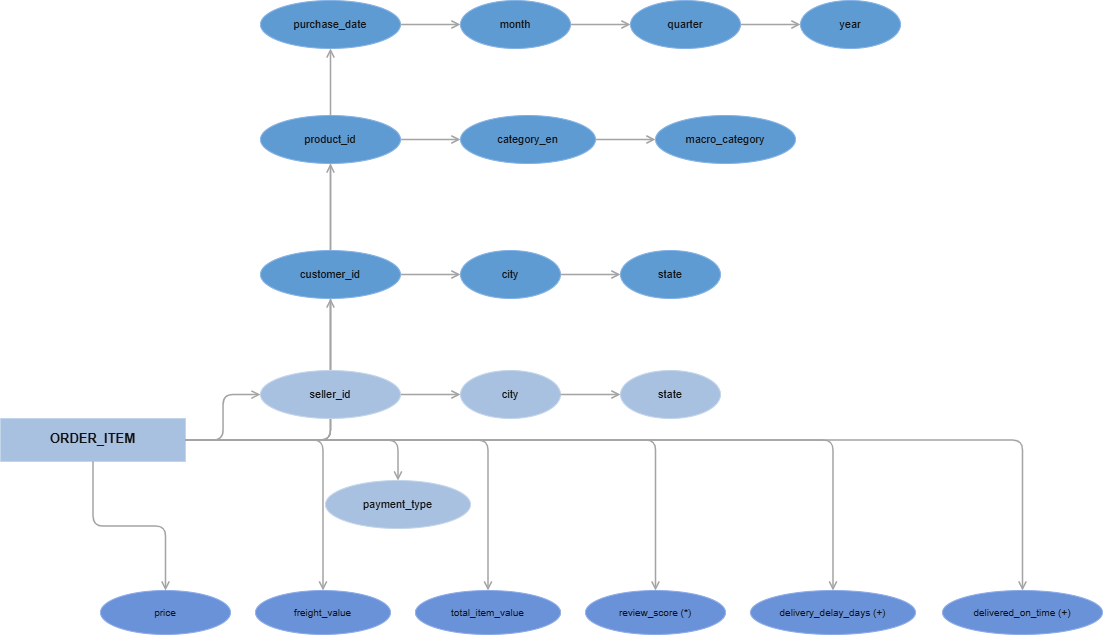
\includegraphics[width=\textwidth]{attribute_tree_pieno.png}
  \caption{Attribute Tree of the \texttt{Order\_Items} fact table}
  \label{fig:attrtree}
\end{figure}

\subsection{From the Attribute Tree to the DFM Schema}

Starting from the attribute tree, I applied the standard data-driven rules to get to
the DFM schema. Main steps:

\begin{enumerate}
  \item \textbf{Picking the dimensions}: the foreign keys (\texttt{product\_id},
        \texttt{seller\_id}, \texttt{customer\_id}, \texttt{payment\_type},
        \texttt{purchase\_date}) became dimensions.

  \item \textbf{Editing the attribute tree}: the DFM method provides two operations.
        \textbf{Pruning} a vertex $v$ means cutting the whole subtree under it --
        those attributes disappear from the fact table and cannot be used for
        aggregation anymore. \textbf{Grafting} a vertex $v$ with parent $v'$ is for
        when $v$ itself is not interesting but its children are worth keeping: $v$'s
        children are connected directly to $v'$ and $v$ is dropped, losing that
        aggregation level but keeping what is below it. Here is what I did:
        \begin{itemize}
        \sloppy
          \item \textit{Pruned \texttt{customer\_unique\_id}}: cut the whole subtree
                (it is a leaf, no children). At single order-item granularity,
                \texttt{customer\_id} is already enough -- keeping both would just
                be redundant.
          \item \textit{Grafted \texttt{zip\_code\_prefix}}: removed this vertex and
                connected its children \texttt{city} and \texttt{state} directly to
                the parent (\texttt{customer\_id}/\texttt{seller\_id}). I lose the
                per-ZIP granularity, which is too fine for the analyses I planned
                anyway, but the $\text{city} \to \text{state}$ hierarchy survives.
          \item \textit{Pruned the free-text Reviews attributes}: cut the whole
                subtree of unstructured text fields, since they are of no use for
                quantitative OLAP analysis. Only \texttt{review\_score} stays as a
                measure.
          \item \textit{Pruned the quality flags}: cut the whole
                \texttt{\_imputed}/\texttt{\_outlier}/\texttt{\_missing} subtree --
                useful for auditing in the reconciled database, but meaningless for
                analysis in the warehouse.
          \item \textit{Added the \texttt{category\_en} $\to$
                \texttt{macro\_category} hierarchy}: the source only gives the
                category in Portuguese, so I added the English translation (already
                available in the reconciled database) plus a macro-category, to
                allow high-level roll-ups. This is not really pruning or grafting,
                more an extension of the tree with a new derived attribute and
                hierarchy.
          \item \textit{Promoted \texttt{payment\_type} to a dimension}: per the DFM
                rules, dimensions come from the direct children of the tree's root.
                Since one order can use several payment methods (e.g.\ voucher $+$
                card), to avoid duplicating rows in the fact table I assigned each
                row the \textbf{payment method of the first installment recorded for
                that order} (in \texttt{rec\_fact\_payments}), while
                \texttt{payment\_value} is the sum of everything paid for the order.
                It is a deterministic choice, but not based on which installment was
                largest -- a natural next step would be a dedicated bridge table for
                multiple payments, avoiding the need to pick a single ``main''
                method.
          \item \textit{\texttt{total\_item\_value} and
                \texttt{delivered\_on\_time}}: these show up as conceptual measures
                in the attribute tree. \texttt{total\_item\_value} $=$
                \texttt{price} $+$ \texttt{freight\_value} is not stored in the fact
                table, since it is trivial to compute on the fly -- it is done
                directly in Tableau. \texttt{delivered\_on\_time} can be derived
                from \texttt{delivery\_delay\_days} $\leq 0$, so it does not need
                its own column in the warehouse.
        \end{itemize}

  \item \textbf{Roll-up hierarchies}:
        \begin{itemize}
          \item \textbf{Time}: day $\to$ month $\to$ quarter $\to$ year
          \item \textbf{Product}: \texttt{product\_id} $\to$ \texttt{category\_en}
                $\to$ \texttt{macro\_category}
          \item \textbf{Customer}: \texttt{customer\_id} $\to$ \texttt{city} $\to$
                \texttt{state} $\to$ \texttt{region}
          \item \textbf{Seller}: \texttt{seller\_id} $\to$ \texttt{city} $\to$
                \texttt{state}
          \item \textbf{Payment}: \texttt{payment\_type} $\to$
                \texttt{payment\_category}
        \end{itemize}

  \item \textbf{Sorting measures by additivity}:
        \begin{itemize}
        \sloppy
          \item \textit{Additive}: \texttt{price}, \texttt{freight\_value} -- can be
                summed along any dimension, item level included;
          \item \textit{Additive only at order level}: \texttt{payment\_value},
                \texttt{payment\_installments} -- these come from an aggregate per
                \texttt{order\_id} (Section~\ref{sec:join-fact-sales}) and get
                copied onto every item row of the same order in
                \texttt{fact\_sales}, so summing them at item level is wrong (one
                would double-count). They need to be aggregated by
                \texttt{order\_id} before a SUM, or used with AVG at item level;
          \item \textit{Non-additive}: \texttt{review\_score} -- AVG only, summing
                scores does not mean anything;
          \item \textit{Semi-additive}: \texttt{delivery\_delay\_days},
                \texttt{delivery\_lead\_days} -- cannot be summed over time (summing
                delays is meaningless), but AVG, MAX, MIN all work fine.
        \end{itemize}
\end{enumerate}

\subsection{Considerations on information loss}

Two design choices come with some controlled loss of detail:

\begin{itemize}
  \item \textbf{Multiple payments}: I aggregate payments by \texttt{order\_id} (sum
        of \texttt{payment\_value} and \texttt{payment\_installments}, plus the main
        payment method) before joining with the order items. That means the detail
        of secondary payment methods is lost. Since the per-order aggregate is
        stamped on every item row, \texttt{payment\_value} and
        \texttt{payment\_installments} are only additive at the order level, not the
        item level (see Section~\ref{sec:join-fact-sales} and
        Table~\ref{tab:misure}).
  \item \textbf{Geolocation}: aggregating by ZIP loses the point-by-point
        variability of the coordinates, which is acceptable since the planned
        analyses work at city/state level anyway. It is worth noting that 278
        customer records (157 distinct ZIP codes) and 7 sellers have no match in
        \texttt{Geolocation}, so \texttt{lat}/\texttt{lng} are NULL for those rows
        in the warehouse -- no real impact on state-level geographic analysis.
\end{itemize}

The resulting DFM schema is shown in Figure~\ref{fig:dfm}.

\begin{figure}[H]
  \centering
  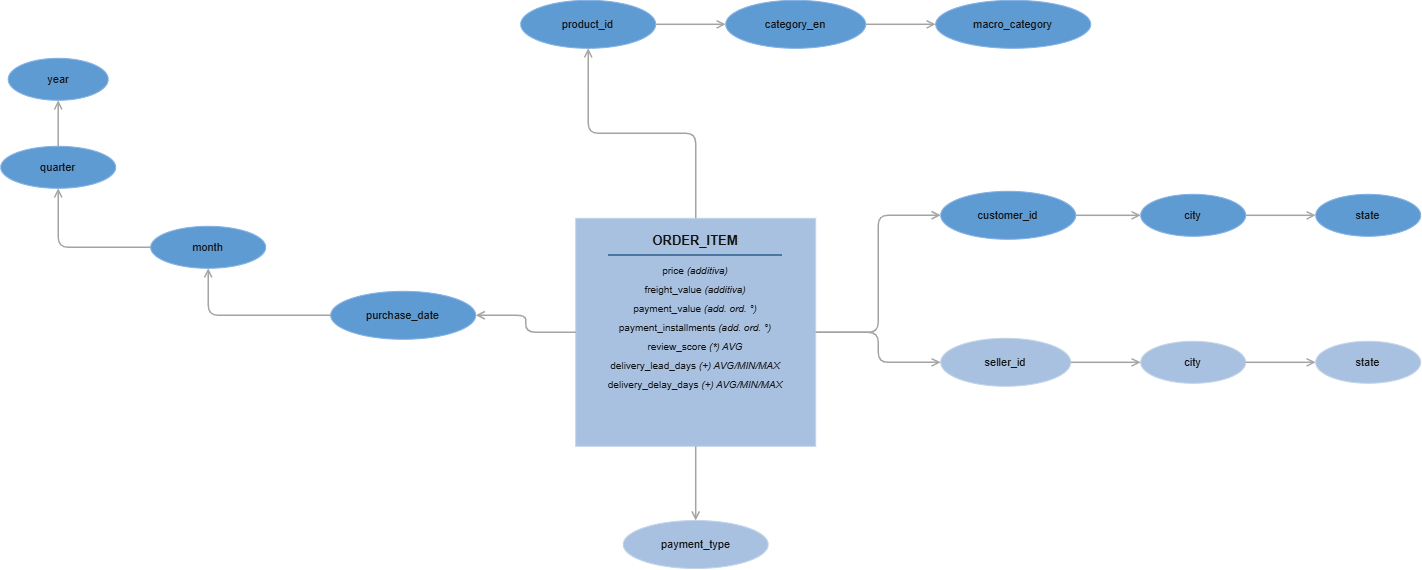
\includegraphics[width=0.85\textwidth]{dfm_schema_pieno_v2.png}
  \caption{DFM Schema of the \texttt{ORDER\_ITEM} fact}
  \label{fig:dfm}
\end{figure}

% ═══════════════════════════════════════════════════════════════════════════
%  5. LOGICAL DESIGN – STAR SCHEMA
% ═══════════════════════════════════════════════════════════════════════════
\section{Logical Design -- Star Schema}

\subsection{Translation from the DFM to the Star Schema}

Each DFM dimension turns into a table with a natural primary key, and the fact table
centralizes the FKs to every dimension plus the measures. I went with a \textbf{star
schema} instead of a snowflake mainly because it keeps OLAP queries simple -- fewer
joins, faster aggregations -- with hierarchies denormalized inside each dimension
table. The star schema is shown in Figure~\ref{fig:star}.

\begin{figure}[H]
  \centering
  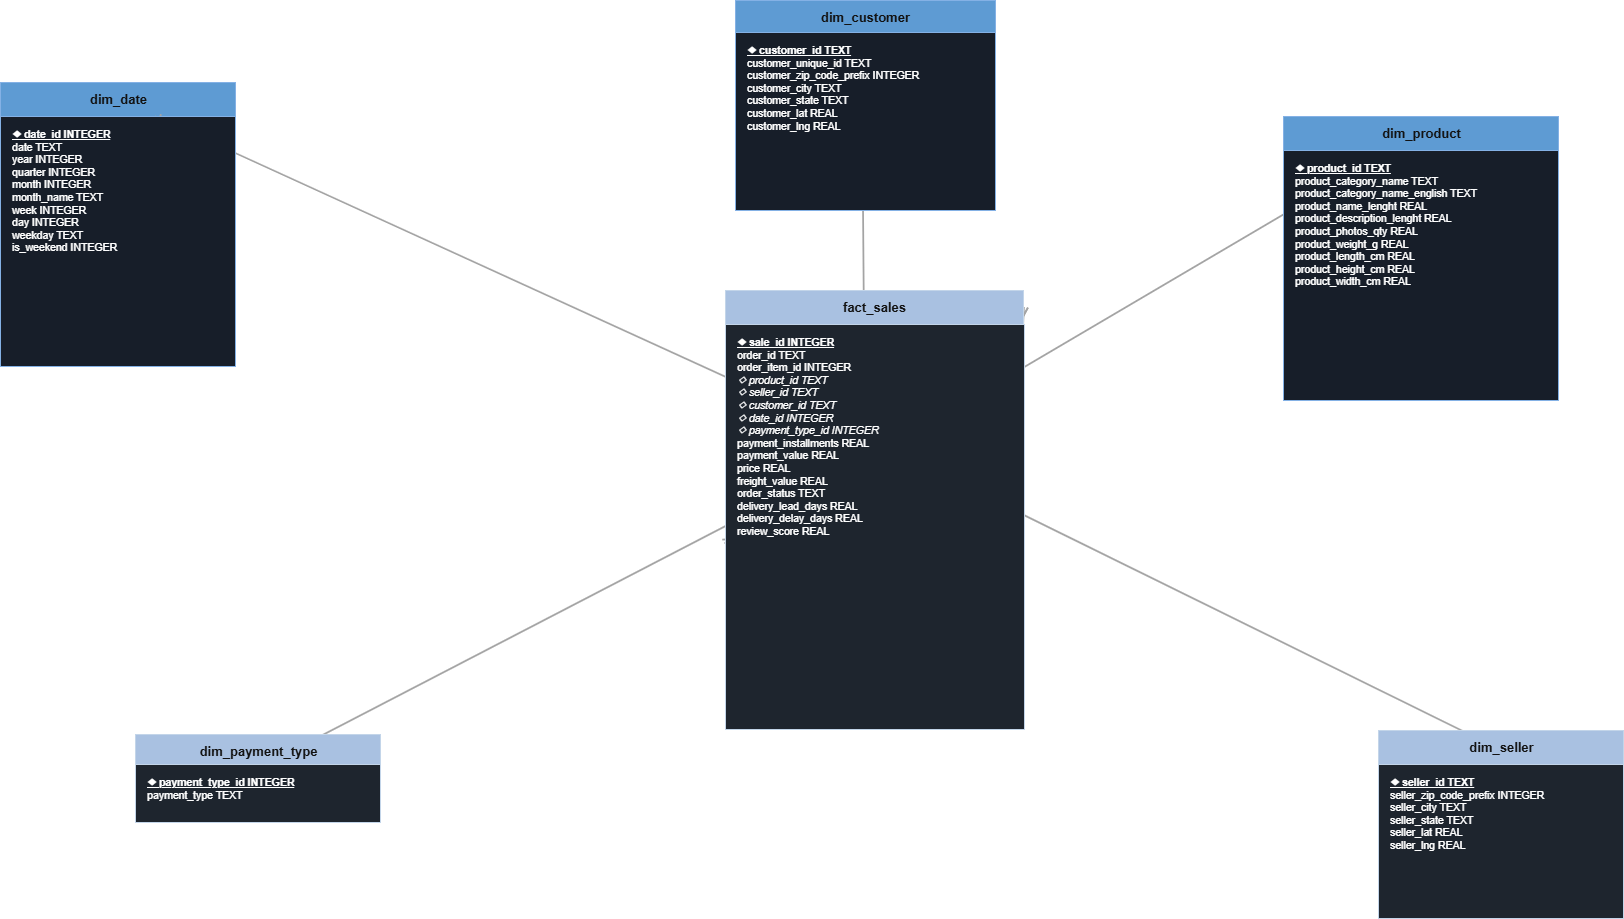
\includegraphics[width=0.85\textwidth]{star_schema_pieno.png}
  \caption{Star Schema of the Olist Data Warehouse}
  \label{fig:star}
\end{figure}

\subsection{Support for OLAP operations}

The model supports the main OLAP operations:

\begin{itemize}
  \item \textbf{Roll-up}: day to month, quarter to year, city to state,
        \texttt{product\_category\_name\_english} to category;
  \item \textbf{Drill-down}: year to quarter, \texttt{category\_en} down to a single
        product;
  \item \textbf{Slice \& Dice}: filtering by state, year, payment type, product
        category.
\end{itemize}

\subsection{Data Warehouse Tables}

\begin{table}[H]
  \centering
  \caption{Structure of the \texttt{fact\_sales} fact table}
  \label{tab:fact}
  \begin{tabular}{lll}
    \toprule
    \textbf{Column} & \textbf{Type} & \textbf{Description} \\
    \midrule
    \texttt{sale\_id}             & INT PK   & Surrogate key of the fact table \\
    \texttt{order\_id}            & TEXT     & Natural key of the order (traceability) \\
    \texttt{order\_item\_id}      & INT      & Progressive number of the item within the order \\
    \texttt{date\_id}             & INT FK   & Reference to \texttt{dim\_date} (YYYYMMDD) \\
    \texttt{product\_id}          & TEXT FK  & Reference to \texttt{dim\_product} \\
    \texttt{customer\_id}         & TEXT FK  & Reference to \texttt{dim\_customer} \\
    \texttt{seller\_id}           & TEXT FK  & Reference to \texttt{dim\_seller} \\
    \texttt{payment\_type\_id}    & INT FK   & Reference to \texttt{dim\_payment\_type} \\
    \texttt{order\_status}        & TEXT     & Order status (degenerate attribute) \\
    \texttt{payment\_installments} & REAL    & Number of payment installments -- additive only at order level (Tab.~\ref{tab:misure}) \\
    \texttt{price}                & REAL     & Product price -- additive measure \\
    \texttt{freight\_value}       & REAL     & Shipping cost -- additive measure \\
    \texttt{payment\_value}       & REAL     & Total payment value -- additive only at order level (Tab.~\ref{tab:misure}) \\
    \texttt{delivery\_lead\_days} & REAL     & Days from sale to delivery -- semi-additive (AVG, MAX, MIN) \\
    \texttt{delivery\_delay\_days} & REAL    & Delay relative to the estimated date (negative = early) -- semi-additive \\
    \texttt{review\_score}        & REAL     & Review score 1--5 -- AVG only (non-additive) \\
    \bottomrule
  \end{tabular}
\end{table}

\textit{Note: \texttt{order\_id} and \texttt{order\_item\_id} stay in the fact table
as degenerate attributes, purely so I can trace back to the operational source
without needing a dedicated dimension. \texttt{payment\_value} and
\texttt{payment\_installments} come from a per-order aggregate and get copied onto
every item row, so they are additive only at the order level, not the item level
(see Table~\ref{tab:misure} and Section~\ref{sec:join-fact-sales}).}

\textbf{Fact table:} \texttt{fact\_sales}

\medskip
\textbf{Dimension tables}

\underline{\texttt{dim\_date}}(date\_id, date, year, quarter, month, month\_name, week, day, weekday, is\_weekend)\\
\textit{Daily granularity. \texttt{date\_id} = YYYYMMDD (e.g.\ 20170913). Supports
roll-up from day up through month, quarter, year. 634 distinct dates covering
2016--2018.}

\medskip
\underline{\texttt{dim\_product}}(product\_id, product\_category\_name,
product\_category\_name\_english, product\_name\_lenght, product\_description\_lenght,
product\_photos\_qty, product\_weight\_g, product\_length\_cm, product\_height\_cm,
product\_width\_cm)\\
\textit{Hierarchy: \texttt{product\_id} $\to$
\texttt{product\_category\_name\_english}. The \texttt{macro\_category} level is
planned in the conceptual DFM but not yet built into the star schema. The column
names \texttt{product\_name\_lenght} and \texttt{product\_description\_lenght} keep
the original source typo, for compatibility.}

\medskip
\underline{\texttt{dim\_customer}}(customer\_id, customer\_unique\_id,
customer\_zip\_code\_prefix, customer\_city, customer\_state, customer\_lat, customer\_lng)\\
\textit{Geographic hierarchy: \texttt{city} $\to$ \texttt{state}. The \texttt{region}
level is planned in the conceptual DFM but not yet built into the current version.}

\medskip
\underline{\texttt{dim\_seller}}(seller\_id, seller\_zip\_code\_prefix, seller\_city,
seller\_state, seller\_lat, seller\_lng)\\
\textit{Geographic hierarchy: \texttt{city} $\to$ \texttt{state}.}

\medskip
\underline{\texttt{dim\_payment\_type}}(payment\_type\_id, payment\_type)\\
\textit{5 values: \texttt{credit\_card} (73.9\%), \texttt{boleto} (19.0\%),
\texttt{voucher} (5.6\%), \texttt{debit\_card} (1.5\%), \texttt{not\_defined}
(0.003\%). Linked to the fact table through each order's main payment method
(aggregated by \texttt{order\_id}), which avoids duplicating rows for orders that
used more than one payment method.}

\subsection{Glossary of measures}
\label{sec:misure}

\begin{table}[H]
  \centering
  \footnotesize
  \caption{Glossary of measures of the \texttt{fact\_sales} fact table}
  \label{tab:misure}
  \begin{tabular}{>{\ttfamily}l
                  >{\raggedright}p{3.5cm}
                  >{\raggedright\arraybackslash}p{5cm}}
    \toprule
    \textbf{Measure} & \textbf{Type / Aggregation} & \textbf{Description} \\
    \midrule
    price                & Additive -- SUM, AVG, MIN, MAX &
      Unit price of the product. Can be summed along any dimension (product,
      customer, seller, time). \\
    freight\_value       & Additive -- SUM, AVG &
      Shipping cost of a single item. Can be summed along any dimension. \\
    payment\_value       & Additive only at order level &
      Total amount paid for the order. \textbf{Warning}: in \texttt{fact\_sales} it
      is copied onto every item row of the same order
      (Section~\ref{sec:join-fact-sales}), so summing it at item level overstates
      the total (19.23M in the DW vs.\ 15.38M in the original payments). Aggregate
      by \texttt{order\_id} first, or use AVG at item level. \\
    payment\_installments & Additive only at order level &
      Number of installments, copied onto every item of the same order for the same
      reason as \texttt{payment\_value}. Aggregate by \texttt{order\_id} before
      analyzing credit usage by category or region. \\
    delivery\_lead\_days & Semi-additive -- AVG, MAX, MIN &
      Days from purchase date to actual delivery. Not summable over time, but
      AVG/MAX/MIN make sense. NULL for undelivered orders. \\
    delivery\_delay\_days & Semi-additive -- AVG, MAX, MIN &
      Delay against the estimated delivery date (negative = early). Not summable
      over time. NULL for undelivered orders. \\
    review\_score        & Non-additive -- AVG only &
      Review score from 1 to 5. Summing it means nothing -- AVG is the only valid
      aggregation. \\
    COUNT(*)             & Count -- SUM &
      Number of items sold. Works along any dimension; equals the number of
      transactions at that granularity. \\
    \bottomrule
  \end{tabular}
\end{table}

\textit{Note on additivity:} \texttt{delivery\_delay\_days} and
\texttt{delivery\_lead\_days} are semi-additive in \texttt{fact\_sales} -- fine with
AVG, MAX, MIN, but not with SUM over time. Both are NULL for orders not yet
delivered (a semantic null, not missing data).

% ═══════════════════════════════════════════════════════════════════════════
%  6. IMPLEMENTATION AND POPULATION (ETL)
% ═══════════════════════════════════════════════════════════════════════════
\section{Implementation and Population (ETL)}

\subsection{ETL Process Architecture}

Going from the reconciled database to the star schema follows the usual ETL process
(\textit{Extract, Transform, Load}), producing the final SQLite database
\texttt{olist\_dw.db}. It is implemented in
\texttt{consegna/2\_scripts/build\_star\_schema.py}, which can run straight from the
cleaned CSVs in \texttt{consegna/3\_cleaned\_data/}: the script rebuilds both the
reconciled layer (\texttt{rec\_*}) and the warehouse layer (\texttt{dim\_*} and
\texttt{fact\_sales}), so the whole process described in this section -- including
the \texttt{payment\_type}/\texttt{payment\_value} aggregation logic from
Section~\ref{sec:join-fact-sales} -- is fully reproducible.
The SQLite database has two distinct layers:

\begin{itemize}
  \item \textbf{Reconciled layer} (\texttt{rec\_*}): the cleaned data, loaded
        straight from the cleaning notebook's CSVs. This is the \textit{operational
        data store} the ETL process reads from to build the warehouse. It keeps all
        the audit columns (\texttt{\_imputed}, \texttt{\_outlier} flags) and the
        derived measures like \texttt{delivery\_delay\_days}.
  \item \textbf{Data warehouse layer} (\texttt{dim\_*} $+$ \texttt{fact\_sales}): a
        star schema built for OLAP queries -- no quality flags, and hierarchies
        denormalized directly into the dimensions.
\end{itemize}

The ETL runs in three phases:

\begin{enumerate}
  \item \textbf{Extract}: read the cleaned CSVs and load them into the reconciled
        layer with \texttt{pandas.to\_sql()} and \texttt{if\_exists=``replace''}.

  \item \textbf{Transform}: build the dimension tables and the fact table from the
        reconciled layer. Specifically:
        \begin{itemize}
          \item The \texttt{dim\_*} tables get populated first, so there are no FK
                violations. Natural keys (\texttt{product\_id},
                \texttt{customer\_id}, etc.) stay as primary keys, which keeps
                everything traceable.
          \item \texttt{dim\_date} is generated on the fly by pulling the distinct
                dates out of the purchase timestamps (\texttt{rec\_orders}) and
                computing year, month, quarter, day, and weekday. It covers
                2016--2018 (634 distinct dates).
          \item \texttt{dim\_customer} and \texttt{dim\_seller} get their
                coordinates (\texttt{lat}/\texttt{lng}) from a LEFT JOIN with
                \texttt{rec\_geolocation} on \texttt{zip\_code\_prefix}.
          \item \texttt{fact\_sales} is built by joining
                \texttt{rec\_order\_items}, \texttt{rec\_orders}, payments
                aggregated per order (\texttt{payment\_value} and
                \texttt{payment\_installments} summed across installments,
                \texttt{payment\_type} taken from the first recorded installment),
                and the average review score per order. Natural keys
                \texttt{order\_id} and \texttt{order\_item\_id} stay as degenerate
                attributes.
        \end{itemize}

  \item \textbf{Load}: load the transformed tables into the final DB
        (\texttt{olist\_dw.db}) with referential integrity turned on
        (\texttt{PRAGMA foreign\_keys = ON}). At this point the DB is ready to be
        queried with analysis and visualization tools.
\end{enumerate}

\subsection{Detail of the JOINs for building \texttt{fact\_sales} and the dimensions}
\label{sec:join-fact-sales}

\texttt{fact\_sales} starts from \texttt{rec\_order\_items} (one row per product per
order) and joins in four sources from the reconciled layer:

\begin{itemize}
\sloppy
  \item \textbf{JOIN with \texttt{rec\_orders}} on \texttt{order\_id}: brings in
        \texttt{customer\_id} and \texttt{date\_id} (obtained by turning
        \texttt{order\_purchase\_timestamp} into the integer YYYYMMDD format).

  \item \textbf{LEFT JOIN with pre-aggregated payments}: before joining, I aggregate
        the payments by \texttt{order\_id} -- \texttt{payment\_value} and
        \texttt{payment\_installments} via \texttt{SUM} across all installments
        regardless of method, and \texttt{payment\_type} from the first recorded
        installment (\texttt{first()}). The LEFT JOIN makes sure order items with no
        recorded payment do not get dropped. \textbf{Side effect}: for orders with
        several items, the per-order total gets copied onto every item row of
        \texttt{fact\_sales}. That is why \texttt{payment\_value} and
        \texttt{payment\_installments} are additive only at the order level and not
        the item level (Table~\ref{tab:misure}): summing \texttt{payment\_value}
        across all of \texttt{fact\_sales} gives 19.23M, vs.\ 15.38M in the original
        per-order payments.

  \item \textbf{LEFT JOIN with pre-aggregated reviews}: reviews are aggregated by
        \texttt{order\_id} with \texttt{AVG(review\_score)}, since an order can get
        more than one rating. The LEFT JOIN also keeps order items with no review.
\end{itemize}

The dimension tables are built like this:

\begin{itemize}
  \item \textbf{\texttt{dim\_customer}} and \textbf{\texttt{dim\_seller}} get their
        geographic coordinates (\texttt{lat}/\texttt{lng}) via a LEFT JOIN with
        \texttt{rec\_geolocation} on \texttt{zip\_code\_prefix}. The LEFT JOIN
        matters here: 278 customer records (157 distinct ZIP codes) and 7 sellers
        are not in \texttt{rec\_geolocation}, and an INNER JOIN would drop those
        records, leaving orphan keys in \texttt{fact\_sales}.

  \item \textbf{\texttt{dim\_date}} is generated on the fly: the code pulls the
        distinct dates from \texttt{rec\_orders.order\_purchase\_timestamp} and
        computes year, month, quarter, day, and weekday for each. The primary key
        \texttt{date\_id} = YYYYMMDD is a sortable, human-readable integer (e.g.\
        20170913).

  \item \textbf{\texttt{dim\_payment\_type}} comes from the distinct values of
        \texttt{payment\_type} in \texttt{rec\_fact\_payments}, each given a
        progressive integer surrogate key. There are 5 values:
        \texttt{credit\_card}, \texttt{boleto}, \texttt{voucher},
        \texttt{debit\_card}, \texttt{not\_defined}.
\end{itemize}

\subsection{Final Data Warehouse Statistics}

\begin{table}[H]
  \centering
  \caption{Final volumes of the Star Schema}
  \label{tab:volumes}
  \begin{tabular}{lrl}
    \toprule
    \textbf{Table} & \textbf{Records} & \textbf{Notes} \\
    \midrule
    \texttt{fact\_sales}        & 112,650 & All order rows with valid operational FKs \\
    \texttt{dim\_customer}      &  99,441 & One record per customer\_id \\
    \texttt{dim\_product}       &  32,951 & Includes English category \\
    \texttt{dim\_seller}        &   3,095 & Includes lat/lng from geolocation \\
    \texttt{dim\_date}          &     634 & 2016--2018 period \\
    \texttt{dim\_payment\_type} &       5 & credit\_card, boleto, voucher, debit\_card, not\_defined \\
    \bottomrule
  \end{tabular}
\end{table}

\textbf{Referential integrity}: checked with control queries on the final DB.
\texttt{fact\_sales} has no orphan rows against \texttt{dim\_product},
\texttt{dim\_seller}, \texttt{dim\_customer}, or \texttt{dim\_date}. For
\texttt{payment\_type\_id}: there are 3 legitimate NULLs, corresponding to the 3
item rows of a single (delivered) order for which the source records no payment at
all -- a known quirk of the Olist dataset; they are not orphan FKs, just a real
state the dataset can be in.

\end{document}
